\documentclass[mstat,12pt]{unswthesis}

\usepackage{color}
\usepackage{fancyvrb}
\newcommand{\VerbBar}{|}
\newcommand{\VERB}{\Verb[commandchars=\\\{\}]}
\DefineVerbatimEnvironment{Highlighting}{Verbatim}{commandchars=\\\{\}}
% Add ',fontsize=\small' for more characters per line
\usepackage{framed}
\definecolor{shadecolor}{RGB}{248,248,248}
\newenvironment{Shaded}{\begin{snugshade}}{\end{snugshade}}
\newcommand{\AlertTok}[1]{\textcolor[rgb]{0.94,0.16,0.16}{#1}}
\newcommand{\AnnotationTok}[1]{\textcolor[rgb]{0.56,0.35,0.01}{\textbf{\textit{#1}}}}
\newcommand{\AttributeTok}[1]{\textcolor[rgb]{0.13,0.29,0.53}{#1}}
\newcommand{\BaseNTok}[1]{\textcolor[rgb]{0.00,0.00,0.81}{#1}}
\newcommand{\BuiltInTok}[1]{#1}
\newcommand{\CharTok}[1]{\textcolor[rgb]{0.31,0.60,0.02}{#1}}
\newcommand{\CommentTok}[1]{\textcolor[rgb]{0.56,0.35,0.01}{\textit{#1}}}
\newcommand{\CommentVarTok}[1]{\textcolor[rgb]{0.56,0.35,0.01}{\textbf{\textit{#1}}}}
\newcommand{\ConstantTok}[1]{\textcolor[rgb]{0.56,0.35,0.01}{#1}}
\newcommand{\ControlFlowTok}[1]{\textcolor[rgb]{0.13,0.29,0.53}{\textbf{#1}}}
\newcommand{\DataTypeTok}[1]{\textcolor[rgb]{0.13,0.29,0.53}{#1}}
\newcommand{\DecValTok}[1]{\textcolor[rgb]{0.00,0.00,0.81}{#1}}
\newcommand{\DocumentationTok}[1]{\textcolor[rgb]{0.56,0.35,0.01}{\textbf{\textit{#1}}}}
\newcommand{\ErrorTok}[1]{\textcolor[rgb]{0.64,0.00,0.00}{\textbf{#1}}}
\newcommand{\ExtensionTok}[1]{#1}
\newcommand{\FloatTok}[1]{\textcolor[rgb]{0.00,0.00,0.81}{#1}}
\newcommand{\FunctionTok}[1]{\textcolor[rgb]{0.13,0.29,0.53}{\textbf{#1}}}
\newcommand{\ImportTok}[1]{#1}
\newcommand{\InformationTok}[1]{\textcolor[rgb]{0.56,0.35,0.01}{\textbf{\textit{#1}}}}
\newcommand{\KeywordTok}[1]{\textcolor[rgb]{0.13,0.29,0.53}{\textbf{#1}}}
\newcommand{\NormalTok}[1]{#1}
\newcommand{\OperatorTok}[1]{\textcolor[rgb]{0.81,0.36,0.00}{\textbf{#1}}}
\newcommand{\OtherTok}[1]{\textcolor[rgb]{0.56,0.35,0.01}{#1}}
\newcommand{\PreprocessorTok}[1]{\textcolor[rgb]{0.56,0.35,0.01}{\textit{#1}}}
\newcommand{\RegionMarkerTok}[1]{#1}
\newcommand{\SpecialCharTok}[1]{\textcolor[rgb]{0.81,0.36,0.00}{\textbf{#1}}}
\newcommand{\SpecialStringTok}[1]{\textcolor[rgb]{0.31,0.60,0.02}{#1}}
\newcommand{\StringTok}[1]{\textcolor[rgb]{0.31,0.60,0.02}{#1}}
\newcommand{\VariableTok}[1]{\textcolor[rgb]{0.00,0.00,0.00}{#1}}
\newcommand{\VerbatimStringTok}[1]{\textcolor[rgb]{0.31,0.60,0.02}{#1}}
\newcommand{\WarningTok}[1]{\textcolor[rgb]{0.56,0.35,0.01}{\textbf{\textit{#1}}}}


%%%%%%%%%%%%%%%%%%%%%%%%%%%%%%%%%%%%%%%%%%%%%%%%%%%%%%%%%%%%%%%%%%
% 
% OK...Now we get to some actual input.  The first part sets up
% the title etc that will appear on the front page
%
%%%%%%%%%%%%%%%%%%%%%%%%%%%%%%%%%%%%%%%%%%%%%%%%%%%%%%%%%%%%%%%%%

\title{Groupe Écotourisme\\[0.5cm]Rapport de projet}

\authornameonly{BRANSOLLE Line, GILIBERT Rémy, GONÇALVES
Hugo, MOHAMEDATNI Aya, SÉNÉCAILLE Cassandra, Triozon Lucas }

\author{\Authornameonly}

\copyrightfalse
\figurespagefalse
\tablespagefalse

%%%%%%%%%%%%%%%%%%%%%%%%%%%%%%%%%%%%%%%%%%%%%%%%%%%%%%%%%%%%%%%%%
%
%  And now the document begins
%  The \beforepreface and \afterpreface commands puts the
%  contents page etc in
%
%%%%%%%%%%%%%%%%%%%%%%%%%%%%%%%%%%%%%%%%%%%%%%%%%%%%%%%%%%%%%%%%%%


%%%%%%%%%%%%%%%%%%%%%%%%%%%%%%%%%%%%%%%%%%%%%%%%%%%%%%%%%%%%%%%%%%%%%%%
%
%  A small sample UNSW Coursework Masters thesis file.
%  Any questions to Ian Doust i.doust@unsw.edu.au and/or Gery Geenens ggeenens@unsw.edu.au
%
%%%%%%%%%%%%%%%%%%%%%%%%%%%%%%%%%%%%%%%%%%%%%%%%%%%%%%%%%%%%%%%%%%%%%%%
%
%  The first part pulls in a UNSW Thesis class file.  This one is
%  slightly nonstandard and has been set up to do a couple of
%  things automatically
%
 
%%%%%%%%%%%%%%%%%
%% Precisely one of the next four lines should be uncommented.
%% Choose the one which matches your degree, uncomment it, and comment out the other two!
%\documentclass[mfin,12pt]{unswthesis}    %%  For Master of Financial Mathematics 
%\documentclass[mmath,12pt]{unswthesis}   %%  For Master of Mathematics
%\documentclass[mstat,12pt]{unswthesis}  %%  For Master of Statistics
%%%%%%%%%%%%%%%%%



\linespread{1}
\usepackage{amsfonts}
\usepackage{amssymb}
\usepackage{amsthm}
\usepackage{latexsym,amsmath}
\usepackage{graphicx}
\usepackage{afterpage}
\usepackage[colorlinks]{hyperref}
\hypersetup{
     colorlinks=true,
     linkcolor=blue,
     filecolor=blue,
     citecolor= black,      
     urlcolor=cyan,
     }
\usepackage{textcomp}
\usepackage{longtable}
\usepackage{booktabs}
\usepackage{float}
\let\origfigure\figure
\let\endorigfigure\endfigure
\renewenvironment{figure}[1][2] {
    \expandafter\origfigure\expandafter[H]
} {
    \endorigfigure
}
\usepackage[T1]{fontenc}
\usepackage{ragged2e}
\def\tightlist{}



%
%  Macros - some of these are in plain TeX (gasp!)
%
\newcommand\blankpage{%
    \null
    \thispagestyle{empty}%
    \addtocounter{page}{-1}%
    \newpage}


%%%%%%%%%%%%%%%%%%%%%%%%%%%%%%%%%%%%%%%%%%%%%%%%%%%%%%%%%%%%%%%%%%
%
%  If you've got some funny special words that LaTeX might not
% hyphenate properly, you can give it a helping hand:
%

\hyphenation{Mar-cin-kie-wicz Rade-macher}


\newlength{\cslhangindent}
\setlength{\cslhangindent}{1.5em}
\newlength{\csllabelwidth}
\setlength{\csllabelwidth}{3em}
\newenvironment{CSLReferences}[2] % #1 hanging-ident, #2 entry spacing
 {% don't indent paragraphs
  \setlength{\parindent}{0pt}
  % turn on hanging indent if param 1 is 1
  \ifodd #1 \everypar{\setlength{\hangindent}{\cslhangindent}}\ignorespaces\fi
  % set entry spacing
  \ifnum #2 > 0
  \setlength{\parskip}{#2\baselineskip}
  \fi
 }%
 {}
\usepackage{calc} % for \widthof, \maxof
\newcommand{\CSLBlock}[1]{#1\hfill\break}
\newcommand{\CSLLeftMargin}[1]{\parbox[t]{\maxof{\widthof{#1}}{\csllabelwidth}}{#1}}
\newcommand{\CSLRightInline}[1]{\parbox[t]{\linewidth}{#1}}
\newcommand{\CSLIndent}[1]{\hspace{\cslhangindent}#1}






\renewcommand{\contentsname}{Table des matières}

\renewcommand{\chaptername}{Chapitre}
\usepackage{changepage}
\usepackage{fancyhdr}
\pagestyle{fancy}
\fancyfootoffset{-2cm}




\begin{document}
\begin{adjustwidth}{-2cm}{}

\beforepreface

%\afterpage{\blankpage}


% Acknowledgements are optional


\prefacesection{Remerciements}

{\bigskip}Nos plus sincères remerciements vont à notre encadrant
pédagogique pour les conseils avisés sur notre travail.\\[1cm] 

{\bigskip\bigskip\bigskip\noindent} 2023-12-22.

%\afterpage{\blankpage}

% Abstract

\prefacesection{Résumé}

résume du projet là

%\afterpage{\blankpage}


\afterpreface





%%%%%%%%%%%%%%%%%%%%%%%%%%%%%%%%%%%%%%%%%%%%%%%%%%%%%%%%%%%%%%%%%%
%
% Now we can start on the first chapter
% Within chapters we have sections, subsections and so forth
%
%%%%%%%%%%%%%%%%%%%%%%%%%%%%%%%%%%%%%%%%%%%%%%%%%%%%%%%%%%%%%%%%%%



%%%%%%%%%%%%%%%%%%%%%%%%%%%%%%%%%%%%%

%\afterpage{\blankpage}


\begin{Shaded}
\begin{Highlighting}[]
\KeywordTok{SELECT} \KeywordTok{id}
\KeywordTok{FROM}\NormalTok{ pays}
\end{Highlighting}
\end{Shaded}

\begin{longtable}[]{@{}l@{}}
\caption{Pays}\tabularnewline
\toprule\noalign{}
id \\
\midrule\noalign{}
\endfirsthead
\toprule\noalign{}
id \\
\midrule\noalign{}
\endhead
\bottomrule\noalign{}
\endlastfoot
AD \\
AE \\
AG \\
AI \\
AL \\
AM \\
AO \\
AR \\
AS \\
AT \\
\end{longtable}

\hypertarget{introduction}{%
\chapter{Introduction}\label{introduction}}

Lorsque les vacances approchent, l'envie de quitter la routine
quotidienne s'accompagne souvent de la recherche d'une destination
idéale. Pour cette étape, plusieurs critères peuvent entrer en compte:
le prix, évidemment, mais aussi le moyen de transport, l'hébergement,
les activités ou encore l'empreinte carbone.

\par

Le tourisme est une activité humaine qui a des impacts multiples et
complexes sur l'environnement, l'économie et la société. Selon
l'Organisation mondiale du tourisme (OMT), le tourisme international a
atteint 1,4 milliard d'arrivées en 2018, soit une croissance de 6 \% par
rapport à l'année précédente. Cette tendance à la hausse devrait se
poursuivre dans les prochaines années, avec une projection de 1,8
milliard d'arrivées en 2030.

\par

En effet, face au changement climatique, de plus en plus de personnes
souhaitent faire attention à impacter le moins possible l'environnement
lors de leurs déplacements. Pendant longtemps, le tourisme a été
appréhendé uniquement au niveau de ses retombées économiques. En 2018,
la consommation touristique représentait 7,4 \% du PIB en France, avec
une croissance dynamique, portée principalement par les visiteurs
étrangers.

\par

Dans le même temps, le secteur engendre de nombreuses pressions sur
l'environnement, et en particulier sur le climat. Selon des données, le
tourisme génère actuellement 11 \% des émissions de gaz à effet de serre
en France. À l'heure où le monde ressent l'urgence de prendre des
mesures significatives face aux défis environnementaux, le secteur du
tourisme émerge comme l'un des contributeurs majeurs aux émissions de
gaz à effet de serre.

\par

Cependant, il n'existe pas de solution simple et universelle pour
concilier tourisme et développement durable. Chaque destination présente
des spécificités et des défis qui nécessitent une analyse approfondie et
une adaptation permanente. C'est pourquoi nous avons créé Écotourisme,
une plateforme en ligne innovante qui propose aux voyageurs une
navigation personnalisée et responsable. Écotourisme se positionne comme
la réponse à cette quête, prenant en compte une variété de critères,
dont le prix, le moyen de transport, et surtout, l'empreinte carbone.

\par

Écotourisme a été conçu pour répondre aux trois besoins principaux de
nos utilisateurs: la réduction des dépenses, la simplification du
processus de voyage, et la promotion de la responsabilité
environnementale. Notre projet joue également un rôle de comparateur
statistique. En effet, en collectant des données, nous présentons des
statistiques couvrant de nombreuses années et divers indicateurs liés à
l'économie, à l'écologie et au tourisme. À l'aide de graphiques et d'un
score ``Ecotourisme'' attribué à chaque pays, les utilisateurs ont accès
à des données globales, continentales et nationales. De plus, il est
possible de comparer les données statistiques entre deux pays et choisir
celui qui correspond le mieux à vos attentes et à vos valeurs. Que vous
soyez un voyageur économe, un éco-voyageur engagé, ou simplement un
passionné soucieux de minimiser son impact sur l'environnement,
Écotourisme est votre solution.

\par

Ce qui distingue fondamentalement notre plateforme est son approche
intégrée. Contrairement à d'autres services qui se concentrent
uniquement sur l'aspect économique ou environnemental, Écotourisme
fusionne ces deux dimensions pour offrir une solution complète. Ce
rapport a pour but de présenter notre projet Écotourisme, une plateforme
qui propose aux voyageurs une offre personnalisée et responsable, basée
sur des données statistiques et des critères économiques et
environnementaux.

\hypertarget{sujet}{%
\chapter{Sujet}\label{sujet}}

Dans cette section du rapport, nous explorerons en détail la
modélisation de notre projet à travers l'utilisation d'UML (Unified
Modeling Language) et du Canvas, ainsi que la définition de nos besoins
et exigences dans le cahier des charges. Ces outils puissants nous
permettront de visualiser et de structurer les différents aspects de
notre projet, offrant ainsi une compréhension approfondie de son
architecture.

Notre projet aborde plusieurs besoins et problèmes clés auxquels sont
confrontés les voyageurs d'aujourd'hui. En premier lieu, nous répondons
à la quête d'économie des voyageurs en les aidant à réduire leurs
dépenses, proposant ainsi une réponse adaptée au voyage économique.
Simultanément, notre initiative s'engage en faveur de la responsabilité
environnementale en encourageant des pratiques de voyage respectueuses
de l'environnement. De plus, notre solution vise à démystifier le
processus de voyage en fournissant des informations claires et
accessibles. En simplifiant les démarches, nous aspirons à rendre
l'expérience de voyage plus transparente et moins intimidante pour nos
utilisateurs. Enfin, notre projet va au-delà de la simple utilité en
encourageant activement le voyage. Nous aspirons à inspirer les
individus à explorer de nouveaux horizons tout en promouvant la
préservation de notre planète. Ainsi, notre approche sert à la fois les
intérêts des voyageurs en quête de simplicité et d'économie, tout en
contribuant à la promotion de pratiques de voyage durables.

Aujourd'hui, plusieurs alternatives existent pour répondre aux besoins
des voyageurs en quête d'économie et de responsabilité environnementale.
Des plateformes de comparaison de voyages telles que Kayak ou Liligo se
concentrent principalement sur l'aspect économique, offrant des options
pour minimiser les coûts des déplacements. D'autre part, des sites comme
l'ADEME, Carbon Footprint, et la Fondation Goodplanet permettent de
calculer l'empreinte carbone associée aux voyages.

Cependant, notre approche se distingue en fusionnant ces deux aspects
cruciaux du voyage. Notre plateforme offre une approche polyvalente en
intégrant la comparaison économique et la mesure de l'empreinte carbone.
En éliminant la nécessité pour les utilisateurs de consulter plusieurs
sites simultanément, notre système simplifie le processus de
planification du voyage, offrant ainsi une expérience complète pour ceux
qui aspirent à voyager de manière économique et écologique. Notre
différenciation réside dans la consolidation de ces fonctionnalités
clés, offrant ainsi une réponse intégrée et pratique pour les voyageurs
soucieux de leur budget et de l'environnement. Notre solution s'adresse
à une diversité d'usagers partageant un intérêt commun pour des voyages
économiques et respectueux de l'environnement. Nous ciblons un large
éventail de personnes, sans distinction d'âge ou de besoins spécifiques.
Les principaux usagers visés comprennent:

\begin{itemize}
\tightlist
\item
  \textbf{Voyageurs économes:} Ceux qui cherchent des moyens efficaces
  de réduire leurs dépenses tout en profitant pleinement de leur
  expérience de voyage.
\item
  \textbf{Éco-voyageurs:} Les individus engagés dans des pratiques de
  voyage respectueuses de l'environnement, souhaitant minimiser leur
  impact écologique tout en explorant le monde. Étudiants et jeunes
  voyageurs: Cette catégorie inclut les étudiants et les jeunes adultes
  à la recherche d'options de voyage abordables et informatives pour
  enrichir leur expérience.
\item
  \textbf{Curieux et passionnés:} Les personnes animées par la curiosité
  et la passion pour la découverte, cherchant des informations claires
  et inspirantes pour leurs voyages. En ciblant ces différents profils,
  notre projet aspire à répondre aux attentes variées de notre public,
  créant ainsi une plateforme inclusive et accessible à tous les
  amateurs de voyages économiques et écologiques.
\end{itemize}

\vskip 1.0em Notre solution, dédiée à l'écotourisme, représente une
plateforme tout-en-un pour des voyages économiques et respectueux de
l'environnement. Elle offre un accès simplifié à une gamme complète
d'informations essentielles, couvrant à la fois l'aspect économique et
écologique des destinations.

Les fonctionnalités clés de notre plateforme incluent la fourniture
d'informations détaillées sur l'économie et l'écologie de chaque
destination, permettant aux utilisateurs de prendre des décisions
informées. De plus, notre système propose un calcul précis de
l'empreinte carbone associée à chaque itinéraire, aidant ainsi les
voyageurs à évaluer et à minimiser leur impact environnemental. En plus
de cela, notre plateforme offre une visibilité sur les coûts de voyage,
facilitant la planification budgétaire des utilisateurs. Enfin, elle
fournit des conseils pratiques pour des choix responsables tout au long
du processus de planification et d'exécution du voyage. En résumé, notre
solution vise à simplifier et à enrichir l'expérience de voyage en
offrant une approche complète, favorisant des voyages économiques et
respectueux de l'environnement. Pour faciliter l'accès aux données, nous
avons mis en place une carte interactive pour la sélection de la région
du monde. En outre, nous intégrerons une barre de recherche munie d'un
système d'autocorrection, permettant aux utilisateurs de trouver
rapidement les informations dont ils ont besoin. Ces fonctionnalités
visent à rendre l'expérience utilisateur fluide et intuitive, offrant un
accès rapide et personnalisé aux données économiques et écologiques.
Pour constituer notre base de données, nous avons réalisé des recherches
approfondies en nous appuyant sur des sources fiables telles que
l'UNWTO, l'ONU, la Banque Mondiale, l'OCDE, et l'UE. Compte tenu de la
diversité des domaines couverts par notre projet, nous avons croisé ces
sources et comparé les données qu'elles fournissent, englobant des
informations variées en économie, en écologie et dans le secteur du
tourisme. En outre, nous avons intégré des données non chiffrées,
notamment des listes de pays, de villes, et des pays en conflit, que
nous avons traitées de manière spécifique. La plupart de ces fichiers
étaient au format xlsx, nécessitant un traitement à l'aide de Python.
Cette approche méthodique garantit la fiabilité et la pertinence des
informations fournies par notre plateforme, renforçant ainsi la qualité
de l'expérience utilisateur.

A présent, nous allons nous intéresser à la modélisation pour mieux
appréhender la complexité et la cohérence de notre initiative. Pour cela
on va s'intéresser à un utilisateur. Il a deux possibilités, soit
s'identifier ou se créer un compte ou alors aller sur le site de façon
anonyme. Si l'utilisateur décide s'identifier,l'utilisateur aura la
possibilité d'estimer son empreinte carbone ainsi que le coût d'un
trajet depuis son domicile jusqu'à une destination spécifique. Cette
fonctionnalité lui permettra d'obtenir rapidement une estimation des
dépenses liées à son voyage tout en développant sa conscience
environnementale. De plus, il peut mettre en favoris ses destinations
favorite ou ses projets de voyage. Ainsi, grâce à la sauvegarde des
informations, l'utilisateur peut garder son historique des calculs et
des trajets mais aussi de ses favoris. Ensuite, un utilisateur connecter
ou non peut lire les rapport d'analyse statistiques basé sur des aspects
économique et/ou écologique. De plus en recherchant une région du monde
ou en comparant différentes données (jusqu'à deux régions du monde
différentes) il pourra visualiser des données en fonction de ces
recherches pour pouvoir mieux s'informer ou mieux décider. Pour
conclure, lors de la conception et du développement de notre plateforme
Ecotourisme, certaines contraintes et limitations cruciales doivent être
prises en compte pour garantir le succès du projet. Les principales
contraintes comprennent:

\begin{itemize}
\tightlist
\item
  \textbf{Conformité aux normes de sécurité:} La plateforme devra
  respecter les normes de sécurité les plus strictes pour assurer la
  confidentialité des données des utilisateurs et garantir une
  expérience en ligne sécurisée.
\item
  \textbf{Synchronisation des différentes avancées de chacun:} En raison
  de la collaboration entre les membres de l'équipe, il est impératif de
  maintenir une synchronisation constante des progrès réalisés par
  chacun. Des mécanismes de communication et de suivi seront mis en
  place pour assurer une collaboration efficace.
\item
  \textbf{Intégration des idées individuelles:} Notre approche
  collaborative inclura l'intégration des idées individuelles de manière
  cohérente dans le développement de la plateforme. Chaque membre de
  l'équipe aura l'opportunité de contribuer de manière significative à
  la conception et à l'amélioration continue.
\item
  \textbf{Adaptation aux emplois du temps de tous:} Compte tenu des
  contraintes d'emploi du temps de chaque membre de l'équipe, des
  mécanismes flexibles seront mis en place pour permettre une
  contribution optimale tout en respectant les engagements
  professionnels et personnels de chacun.
\item
  \textbf{Résolution des problèmes techniques sur le site:} Tout
  problème technique sur la plateforme sera traité de manière rapide et
  efficace. Nous collaborons activement pour identifier l'origine du
  problème et le résoudre promptement. Processus de conception et
  d'imagination du site: Le processus de conception et d'imagination du
  site sera continu et itératif. Les membres de l'équipe auront la
  possibilité de contribuer à l'évolution constante du site, favorisant
  ainsi la créativité et l'innovation.
\end{itemize}

Ces contraintes et limitations guideront notre équipe tout au long du
projet, garantissant que notre plateforme Ecotourisme répondra aux
normes les plus élevées, tout en restant flexible et innovante dans sa
conception et son développement.

\hypertarget{base-de-donnuxe9es}{%
\chapter{Base de données}\label{base-de-donnuxe9es}}

\hypertarget{duxe9veloppement-et-outils}{%
\chapter{Développement et outils}\label{duxe9veloppement-et-outils}}

\hypertarget{planning}{%
\chapter{Planning}\label{planning}}

\textbf{Rapport d'Avancement du Projet}

\hypertarget{introduction-1}{%
\section{Introduction}\label{introduction-1}}

La planification d'un projet demeure un élément crucial pour assurer une
progression efficace et la réussite du projet. Nous avons mis en place
un planning, en prenant en compte les ajustements nécessaires pour
répondre aux éventuels défis rencontrés. Nous avons utilisé Mindview
pour fournir une visualisation claire des tâches et des dépendances. Le
diagramme généré a été d'une grande valeur pour la communication interne
et ont facilité la compréhension des membres de l'équipe sur les
différentes phases du projet. Ainsi il nous servira à illustrer ce
rapport.

\hypertarget{global}{%
\section{Global}\label{global}}

\begin{figure}
\centering
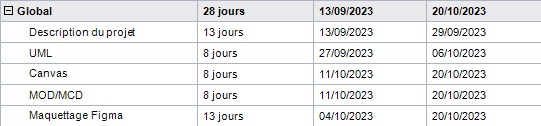
\includegraphics[width=12cm,height=1.34cm]{images/global_gantt.png}
\caption{Diagramme de Gantt global}
\end{figure}

Au cours des premiers cycles du projet, l'équipe a consacré une
attention particulière à plusieurs phases clés, conformément au planning
initial. Les activités suivantes ont été menées avec succès, contribuant
à l'avancement global du projet:

\begin{itemize}
\item
  \textbf{Description du Projet (13 jours):} Les réunions de travail ont
  permis de définir clairement les objectifs et les besoins
  d'écotourisme. Pour avoir une vision plus globale et claire.
\item
  \textbf{Modélisation UML (8 jours):} Dans cette phase, l'équipe a
  consacré huit jours à la création de modèles UML détaillés. Ces
  modèles ont servi de fondement conceptuel, facilitant la visualisation
  des différentes composantes site.
\item
  \textbf{Élaboration du Canevas (8 jours):} Le canevas du projet,
  fournie une représentation visuelle de l'architecture globale. Cette
  étape a permis de valider les besoins du projet avant de passer à des
  phases plus détaillées.
\item
  \textbf{Conception MCD/MOD (8 jours):} Huit jours ont été alloués à la
  conception du Modèle Conceptuel de Données (MCD) et du Modèle
  Organisationnel de Données (MOD). Ces modèles ont permis de définir la
  structure des données et les relations, guidant ainsi le développement
  ultérieur.
\item
  \textbf{Maquettage avec Figma (13 jours):} Comme décrit plus tôt la
  phase de maquettage avec Figma a occupé treize jours, pendant lesquels
  l'équipe a créé des maquettes interactives et visuelles du projet.
  Même si le temps de réalisation en nombre de jour est similaire aux
  autres tâches, celle-ci nous a demandé un investissement plus
  important, par la quantité de travail qu'elle représente. Élaborer un
  diagramme n'est pas comparable à imaginer une dizaine de pages Web, et
  le résultat a été obtenu par une concentration particulière de tous
  nos moyens sur cet objectif.
\end{itemize}

Ainsi comme montré sur l'image plus tôt la mise en place avant codage
nous a pris 1 mois complet afin de cerner l'entièreté des enjeux de ce
projet. On remarque aussi que l'organisation de notre groupe nous a
permis de travailler en différé sur ces taches et ainsi de gagner un
temps précieux.

\newpage

\hypertarget{partie-base-de-donnuxe9es}{%
\section{Partie Base de Données}\label{partie-base-de-donnuxe9es}}

\begin{figure}
\centering
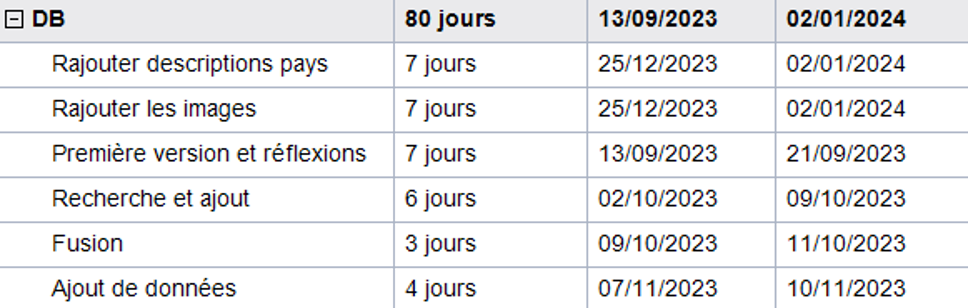
\includegraphics[width=12cm,height=3.82cm]{images/db_gantt.png}
\caption{Diagramme de Gantt Base de données}
\end{figure}

La gestion évolutive de la base de données a été une composante cruciale
du développement du projet, consolidant progressivement les données
touristiques et économiques pour offrir une expérience riche et
complète. Voici un aperçu détaillé des différentes étapes de
développement dans la partie base de données:

\begin{itemize}
\tightlist
\item
  \textbf{13/09 - 21/09:} Au cours de cette phase initiale, la première
  version de la base de données a été élaborée, avec un accent
  particulier sur les données touristiques et les informations
  essentielles sur chaque pays. Des réflexions approfondies ont orienté
  la conception initiale pour garantir une fondation solide.
\item
  \textbf{21/09 - 30/09:} Recherche et Ajout de Données Complémentaires,
  Économie, Écologie et Sûreté, Mise en Place des Clés Étrangères (9
  jours) La base de données a été enrichie par des données
  complémentaires, notamment des informations sur l'économie, l'écologie
  et la sûreté des pays. Les clés étrangères ont été soigneusement mises
  en place pour établir des relations significatives entre les
  différentes tables.
\item
  \textbf{02/10 - 09/10:} Réflexion et Ajouts Mineurs: PIB/hab,
  Continents, Emojis (8 jours) Cette période a été consacrée à des
  réflexions approfondies, conduisant à des ajouts mineurs mais
  significatifs tels que le PIB par habitant, la classification par
  continents et l'introduction d'emojis pour représenter les drapeaux de
  nos pays afin d'obtenir une expérience utilisateur plus visuelle et
  intuitive.
\item
  \textbf{09/10 - 11/10:} Fusion des Tables par Thèmes (2 jours) Une
  étape importante a été la fusion des tables par thèmes, améliorant
  ainsi la cohérence et la facilité d'accès aux données. Cette
  restructuration a contribué à simplifier la gestion de la base de
  données et à rendre les requêtes plus efficientes.
\item
  \textbf{07/11 - 12/11:} Ajout des Données sur les Aéroports et les
  Routes Aériennes (6 jours) L'expansion de la base de données a
  continué avec l'intégration de données sur les aéroports et les routes
  aériennes. Cette addition a considérablement enrichi le volet
  logistique du projet, offrant aux utilisateurs des informations
  détaillées sur les infrastructures aériennes. Ajout d'Images pour
  Chaque Pays: La base de données sera étendue pour inclure des images
  associées à chaque pays, améliorant ainsi l'expérience utilisateur en
  offrant une représentation visuelle.
\item
  \textbf{Gestion Continue:} En reconnaissance du caractère dynamique de
  la base de données, une approche agile sera maintenue pour permettre
  des mises à jour régulières en fonction des besoins changeants du
  projet écotourisme.
\end{itemize}

\newpage

\hypertarget{carte}{%
\section{Carte}\label{carte}}

\begin{figure}
\centering
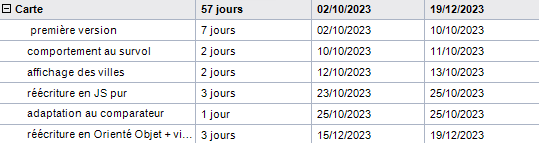
\includegraphics[width=12cm,height=3.21cm]{images/map_gantt.png}
\caption{Diagramme de Gantt: Carte}
\end{figure}

\begin{itemize}
\tightlist
\item
  \textbf{02/10 - 10/10:} Première Version (Fond de Carte, Tests) (9
  jours) Durant cette période, l'équipe a concentré ses efforts sur la
  création de la première version de la carte. C'était la première fois
  que nous approchions cet outil, et la création de cette version
  initiale visait à explorer les fonctionnalités offertes et à évaluer
  sa pertinence. Cette étape préliminaire était importante pour prendre
  une décision sur l'utilisation de l'outil, ce qui a confirmé notre
  choix de poursuivre avec amCharts.
\item
  \textbf{10/10 - 11/10:} Comportement au survol (HTML des Mini-Cartes,
  Tests) (2 jours) La seconde phase du développement, centrée sur le
  comportement au survol, s'est basée sur les premiers bandeaux réalisés
  pour la page pays. En utilisant ces éléments comme référence, l'équipe
  a rédigé le code HTML derrière l'affichage des mini-maps au survol
  (pays change de couleur au survol), renforçant ainsi l'interface
  utilisateur.
\item
  \textbf{12/10 - 13/10:} Affichage des Villes, Focus sur un Pays (2
  jours) Ces deux jours ont été consacrés à l'extension des
  fonctionnalités du projet, notamment l'affichage des villes et la
  fonction de mise en évidence d'un pays spécifique. Ces ajouts
  enrichissent l'expérience utilisateur en fournissant des informations
  un peu plus détaillées sur les différentes pays.
\item
  \textbf{23/10 - 25/10:} Réécriture en JS Pur (3 jours) Une évolution
  majeure a eu lieu avec la réécriture du code en JavaScript pur. Cette
  transition vers un fichier séparé permet de réutiliser la carte dans
  n'importe quelle page souhaitée, anticipant notamment notre future
  page comparateur. Ce qui renforce l'efficacité du développement et la
  maintenance à long terme.
\item
  \textbf{25/10:} Adaptation au Comparateur (Comportement au Clic pour
  Deux Pays) (1 jour) Pour rendre le projet plus polyvalent, des
  ajustements ont été apportés pour permettre le support de deux pays
  mis en avant au lieu d'un seul. Ces modifications s'alignent avec
  notre vision d'extension future du projet vers une page comparateur
  entre pays.
\item
  \textbf{15/12 - 17/12:} Réécriture en Orienté Objet + Villes
  Dynamiques au Clic (3 jours) Une refonte majeure a été entreprise en
  adoptant une approche orientée objet. Inspirée par l'architecture POO
  mise en place pour les graphiques, cette transition améliore la
  lisibilité du code, favorise la réutilisation des fonctionnalités, et
  simplifie la gestion des futures évolutions du projet.
\end{itemize}

\newpage

\hypertarget{page-pays-monde-comparateur}{%
\section{Page Pays/ Monde/
Comparateur}\label{page-pays-monde-comparateur}}

\begin{figure}
\centering
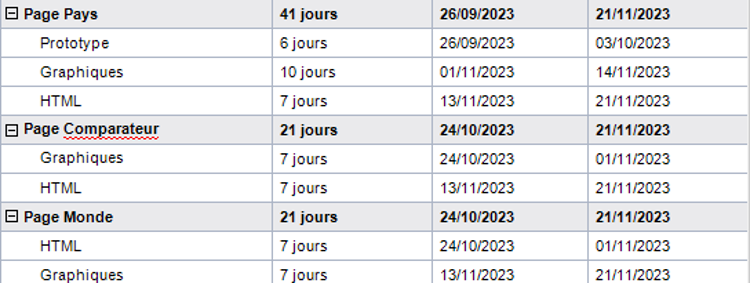
\includegraphics[width=12cm,height=4.52cm]{images/html_gantt.png}
\caption{Diagramme de Gantt: Pages Pays/Monde/Comparateur}
\end{figure}

Chaque page, caractérisée par des fonctionnalités graphiques avancées, a
fait l'objet d'un travail en binôme, favorisant la collaboration et la
génération d'idées innovantes. Initialement planifiées sur une plage de
21 à 41 jours, ces périodes ont été recalculées et étendues jusqu'au 22
décembre en raison de contraintes imprévues. (Partiels et difficultés
sous-estimées).

\textbf{Page Pays:} La page pays a été conçue pour offrir une expérience
approfondie, avec des graphiques détaillés reflétant diverses données
économiques, touristiques et environnementales. \textbf{Page Monde:} La
complexité des graphiques de la page Monde, agrégeant des données de
multiples pays, a demandé une période étendue pour garantir une
représentation précise.

\hypertarget{page-comparateur}{%
\section{Page Comparateur}\label{page-comparateur}}

La page comparateur, met en œuvre des graphiques comparatifs entre deux
pays, a exigé une période supplémentaire pour perfectionner les
interactions utilisateur. L'extension a permis d'affiner les
fonctionnalités de comparaison, d'ajuster les détails visuels et de
garantir une expérience plus fluide.La mise en œuvre de fonctionnalités
graphiques avancées a aussi été mis en place.

\hypertarget{pages-annexes}{%
\section{Pages annexes}\label{pages-annexes}}

\begin{figure}
\centering
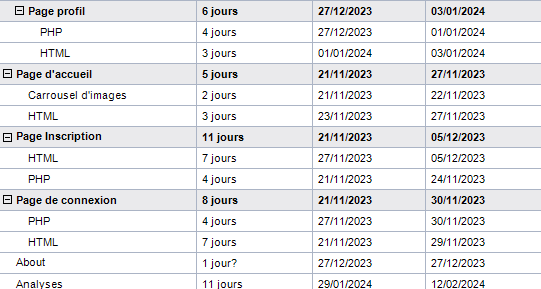
\includegraphics[width=12cm,height=6cm]{images/annex_gantt.png}
\caption{Diagramme de Gantt: Pages annexes}
\end{figure}

La conception et le développement des pages Profil, Inscription,
Connexion, About, Catalogue des Pays, ainsi que la Footer/Navbar ont été
impactés par les ajustements précédents. Ces pages étaient initialement
planifiées entre le 21 novembre et le 3 janvier. Ici la collaboration en
binôme se poursuivra. Voici un les tâches à accomplir au cours de cette
période:

\begin{itemize}
\tightlist
\item
  \textbf{Page Profil (18/12 - 15/01):} Cette page centrale accueillera
  les fonctionnalités de gestion de profil utilisateur, offrant une
  expérience personnalisée.
\item
  \textbf{Pages d'Inscription et de Connexion (18/12 - 15/01):} Ces
  pages seront créées pour une inscription et une connexion sécurisée.
\item
  \textbf{Page About (18/12 - 15/01):} La page About bénéficiera
  également d'ajustements pour refléter les dernières améliorations
  apportées aux autres pages. La période étendue permettra d'approfondir
  la présentation du projet, de l'équipe et des objectifs globaux.
\item
  \textbf{Catalogue des Pays (18/12 - 15/01):} La création du catalogue
  des pays facilitera la navigation à travers les informations, offrant
  une expérience plus rapide et conviviale. Cette fonctionnalité
  optimisera la recherche d'informations spécifiques sur les différents
  pays / continent présents dans la base de données.
\item
  \textbf{Footer/Navbar (18/12 - 15/01):} Le Footer et la Navbar, seront
  ajustés pour assurer une navigation intuitive sur l'ensemble du site.
  Les liens vers les différentes pages, y compris les nouvelles, seront
  intégrés de manière cohérente.
\end{itemize}

\newpage

\hypertarget{derniuxe8re-pages-et-enjeux-cruciaux}{%
\section{Dernière pages et enjeux
cruciaux}\label{derniuxe8re-pages-et-enjeux-cruciaux}}

Au cours de la période s'étendant du 15 janvier au 29 janvier, les
efforts de développement seront concentrés sur la création des pages
Continent et Calculateur. Parallèlement, un contrôle qualité exhaustif
sera effectué sur l'ensemble des pages du site pour garantir une
expérience utilisateur homogène. Ces pages ont également été affectées
par les ajustements de planning antérieurs.

\begin{itemize}
\tightlist
\item
  \textbf{Page Continent (15/01 - 29/01):} La page Continent a été
  conçue pour offrir une expérience approfondie, avec des graphiques
  détaillés reflétant diverses données économiques, touristiques et
  environnementales, elle est proche de la page pays.
\item
  \textbf{Page Calculateur (15/01 - 29/01):} La page Calculateur, semble
  complexe, mais sera développée pendant cette période. Le calcul de
  l'indice, le contrôle qualité des résultats, et l'ajustement visuel
  seront les priorités. La précisions des calcule est pour nous un enjeu
  majeur de notre projet car sans cela notre site per une grande partie
  de son utilité.
\item
  \textbf{Contrôle Qualité Global (15/01 - 29/01):} Simultanément au
  développement des nouvelles pages, un contrôle qualité complet sera
  réalisé sur l'ensemble du site. Chaque page sera passée en revue pour
  s'assurer de la cohérence des styles CSS, de la précision des
  fonctionnalités, et de la fluidité de l'expérience utilisateur. Des
  ajustements seront apportés si nécessaire.
\end{itemize}

\hypertarget{conclusion-planning}{%
\section{Conclusion planning}\label{conclusion-planning}}

Nous avons rencontré des difficultés imprévues, notamment des
contraintes de temps dues à la complexité des tâches ainsi qu'aux
facteurs externes (examens\ldots) ainsi des ajustements ont été
nécessaires. Chaque membre de l'équipe s'est investi dans des domaines
spécifiques (pages différentes sur fonctionnement de binôme et tâches
annexes), permettant une meilleure efficacité. La collaboration en
binôme a renforcé la créativité et la résolution de problèmes,
favorisant ainsi de meilleurs résultats. À l'approche de la phase finale
du projet, nous restons résolus à surmonter les obstacles restants et à
livrer un site final répondant aux normes élevées que nous avons fixées.

\hypertarget{conclusion}{%
\chapter{Conclusion}\label{conclusion}}

Pour conclure ce rapport, Écotourisme se dresse comme une réponse
novatrice aux défis environnementaux posés par l'industrie du tourisme.
À l'heure où ce secteur contribue de manière significative aux émissions
de gaz à effet de serre, notre plateforme incite à une approche plus
responsable du voyage.

\par

Notre engagement en faveur d'un tourisme responsable se manifeste à
travers une approche intégrée. Écotourisme n'est pas seulement une
plateforme économique, mais un écosystème complet où le plaisir du
voyage coexiste avec la responsabilité écologique. Ce rapport, subdivisé
en plusieurs parties clés, témoigne de notre engagement envers la
transparence. À travers la présentation des objectifs, de la base de
données, du développement, et des outils, nous partageons chaque étape
de notre parcours. Lors de la conception et du développement de notre
plateforme Ecotourisme, certaines contraintes et limitations cruciales
ont été prises en compte pour garantir le succès du projet. Ces
contraintes et limitations guideront notre équipe tout au long du
projet, garantissant que notre plateforme ``Ecotourisme'' répondra aux
normes les plus élevées, tout en restant flexible et innovante dans sa
conception et son développement.

\par

La section dédiée à l'empreinte carbone souligne l'importance cruciale
de comprendre les conséquences environnementales de nos choix de
déplacement. En mettant en lumière les émissions de CO2 associées à
différents trajets, nous avons souhaité éduquer nos utilisateurs et les
inciter à des choix de voyage plus durables.

\par

Écotourisme n'est pas simplement une plateforme de voyage, mais une
invitation à repenser la manière dont nous explorons le monde. Nous
croyons en un avenir où le plaisir du voyage s'aligne avec la
préservation de notre planète.

\par

Ensemble, avec nos utilisateurs, et la communauté mondiale, nous
façonnons un avenir du tourisme plus respectueux, plus vert, et plus
durable. Rejoignez-nous dans cette aventure vers un monde où chaque
voyage compte, non seulement pour nous, mais aussi pour les générations
futures. Voyagez avec conscience. Voyagez avec Écotourisme.





\end{adjustwidth}
\end{document}

